%System Design

\chapter{Impementation}
In this chapter we describe the framework and application implementation. We refer to the technologies we used and their interaction. In some cases we cite some crucial code chunks and explain them. Initially we describe the REST API and we analyze its contents. After an extensive illustration of the back end tier of the framework, we emphasize in the front end. There we mention the technologies that are used and their implementation. Alongside the front end description, we present some fragments of front end use cases.

\section{General JavaScript practices and patterns}
\begin{figure}
	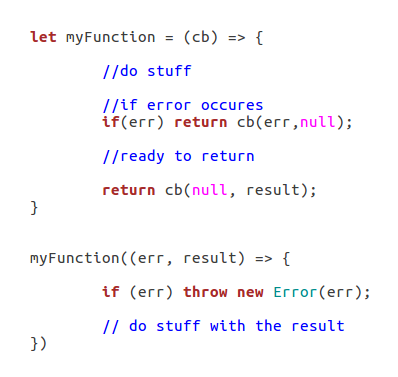
\includegraphics[scale=0.7]{cb.png}
	\caption{Example of a callback function}
	\label{cb}
\end{figure} 
In the framework we developed, we make use of javascript in both front and back end. This programming language uses asynchronous logic, which takes place through the usage of asynchronous callback functions. A callback function is a method which receives as an argument another method, in order to call it later. The execution of the first function does not block the execution of the rest of the program commands. When the execution of the first function ends, the execution of the callback function begins. An example of a callback function can be seen in figure ~\ref{cb}. \par
	In our framework, the callback functions are used constantly, thus the design and implementation are transformed accordingly. As a convention, all the callback functions receive as arguments two objects, the error and the result. Before the execution of the callback function, in case an error occures, the execution stops and the error object is passed to the callback. The result object is obviously null. If no errors occure, the error object is null and the result object contains the function outcome. Next we describe two design patterns, which are based in callback functions and are heavily used in the framework implementation.

\subsection{Closures}
\begin{figure}
	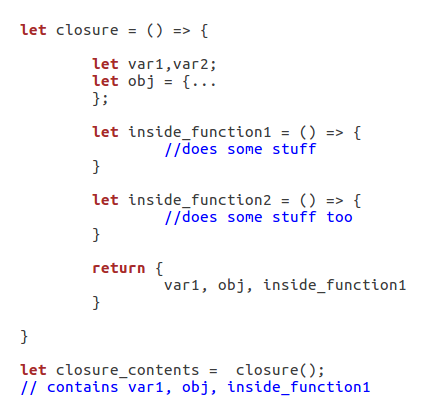
\includegraphics[scale=0.7]{closure.png}
	\caption{Example of a closure function}
	\label{closure}
\end{figure} 
Javascript is an object oriented language and is created to perform well in any platform. Thus, it has many ways of defining certain structures, such as classes. In our framework, we define our classes through the closure design pattern. Closures fully implement a class functionality.\par
	Genarally, a closure in javascript is a function. This function receives arguments that initialize its state. The function body defines its contents, such as variables, objects and other functions. In the end the function returns, or exposes in the rest of the framework, only what is necessary. This may include also variables, objects and functions. Everything that is not returned, equals to what classes define as private. An example of this pattern is shown in figure ~\ref{closure}.

\subsection{Thunks}
\begin{figure}
	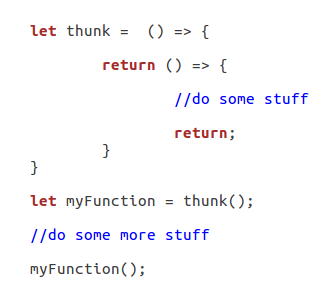
\includegraphics[scale=0.7]{thunk.png}
	\caption{Example of a thunk function}
	\label{thunk}
\end{figure} 
The thunk pattern has a similar structure with closure, but its used in a different way. Basically, its a function which returns another function. The intersting part is that the execution of the first function does not imply the execution of the second. This way we define lazy functions, meaning methods which are scheduled to execute, but they are not until they have to. This pattern is important for solving a problem that occures in javascript, known as callback hell. This problem takes place due to the generation of large sequence of nested callback functions, which is considered a bad design practice and creates debug problems. An example of the thunk pattern is shown in figure ~\ref{thunk}.

\section{Back-End implementation}
Se auto to section estiazoume sto implementation tou back end kommatiou tou framework. Arxika ginetai mia analutiki parousiasi tou REST API pou ulopoiithike kai stin sunexeia perigrafoume to pws ulopoiithikan ta kuriotera modules tou backend. Ektos apo tis texnologies pou xrisimopoiithikan, tha eksigisoume to pws akrivws leitourgoun, ws oloklirwmena modules.

\section{REST API}

